CP2K placeholder text.

What follows is a series of queries for particular kinds of questions of interest that were driven by the needs of CP2K as well as within the \acs{OLCF}.
This is not intended to be a form of definitive analysis to provide specific solutions to problems, but rather a means to create a few classes of representative queries that we expect to be of general use for any user code or system administration.
We start with some queries that require only the output from the compiler and thus are immediately compatible with the normal XALT workflow, then proceed to demonstrate the full power of the tool with a more complex query that makes use of all the different sources of information available to the tool.
However, all of these queries can be easily modified to work on different fields/attributes, combined, or broken apart in any number of ways, as well as made with or without the use of the code sampling frequencies obtained from user profiling to narrow the search space.

\subsection{Determining Use of System and User Libraries}
One of the bigger concerns for system administrators and vendors alike is determining which system resources, particularly that of libraries, are actively being used in applications so as to better direct their focus and efforts.
As such, it is valuable to query not just which libraries are linked in (which has already been done by previous tools like XALT), but also which functions within those libraries are actually getting called within user code.
To this end, we queried CP2K to discover which \ac{FFTW} functions were actually referenced in the code.
The query can be seen in Listing~\ref{lst:fftw}, which simply searches all code statements of type 10 (EXEC\_CALL) and joins each one with the \texttt{gfc\_symbol} table on its \texttt{resolved\_sym} field, which is used for referencing the called function's symbol, before finally outputting a sorted list of all distinct names found for symbols originating from the library module \texttt{fftw3\_lib}.
The results can be seen in Table~\ref{tab:fftw-funcs}.

\begin{lstlisting}[caption=Querying for Use of Library Functions, label=lst:fftw]
select distinct sym.name
from   gcc.gfc_code as code
       join gcc.gfc_symbol as sym
         on sym.record_address = code.resolved_sym
            and sym.build_id = code.build_id
where  code.op = 10
       and sym.module = 'fftw3_lib'
order  by sym.name;
\end{lstlisting}

\begin{table}[htbp]
\caption{FFTW Subroutines Referenced}
\begin{center}
\begin{tabular}{|c|}
\hline
\textbf{Subroutine} \\
\hline
fftw31dm \\
\hline
fftw33d \\
\hline
fftw3\_compute\_rows\_per\_th \\
\hline
fftw3\_create\_3d\_plans \\
\hline
fftw3\_create\_guru\_plan \\
\hline
fftw3\_create\_plan\_1dm \\
\hline
fftw3\_create\_plan\_3d \\
\hline
fftw3\_destroy\_plan \\
\hline
fftw3\_do\_cleanup \\
\hline
fftw3\_do\_init \\
\hline
fftw3\_get\_lengths \\
\hline
fftw3\_workshare\_execute\_dft \\
\hline
fftw\_cleanup \\
\hline
fftw\_export\_wisdom\_to\_file \\
\hline
fftw\_import\_wisdom\_from\_file \\
\hline
sortint \\
\hline
\end{tabular}
\label{tab:fftw-funcs}
\end{center}
\end{table}

The same general form of query could be narrowed down in a couple other ways as well.
In addition to filtering function symbols by module(s), one could also filter based on which file(s) they are found in, or even simply by a chosen set of names.
A user may also want to know more detailed information about invocations, particularly the file/line locations each can be found at.
Table~\ref{tbl:scalapack-funcs} shows an example of exactly this, showing the file and line number or numbers (when the statement spans multiple lines) found for calls to ScaLAPACK subroutines.
The results have been limited to the top 15 for brevity.

\begin{table}[htbp]
\caption{ScaLAPACK Subroutine Reference Locations}
\begin{center}
\begin{tabular}{|c|c|c|}
\hline
\textbf{File} & \textbf{Lines} & \textbf{Subroutine} \\
\hline
src/cp\_dbcsr\_cholesky.F & {103} & pspotrf \\
\hline
src/cp\_dbcsr\_cholesky.F & {105} & pdpotrf \\
\hline
src/cp\_dbcsr\_cholesky.F & {187} & pspotri \\
\hline
src/cp\_dbcsr\_cholesky.F & {189} & pdpotri \\
\hline
src/fm/cp\_cfm\_basic\_linalg.F & {411} & pzgetrf \\
\hline
src/fm/cp\_cfm\_basic\_linalg.F & {703} & pzgetrf \\
\hline
src/fm/cp\_cfm\_basic\_linalg.F & {736,737} & pzgetrs \\
\hline
src/fm/cp\_cfm\_basic\_linalg.F & {799,800} & pzgetrf \\
\hline
src/fm/cp\_cfm\_basic\_linalg.F & {812,813} & pzgetri \\
\hline
src/fm/cp\_cfm\_basic\_linalg.F & {818,819} & pzgetri \\
\hline
src/fm/cp\_cfm\_basic\_linalg.F & {882} & pzpotrf \\
\hline
src/fm/cp\_cfm\_basic\_linalg.F & {938} & pzpotri \\
\hline
src/fm/cp\_cfm\_basic\_linalg.F & {1147} & pztrtri \\
\hline
src/fm/cp\_cfm\_diag.F & {90,91} & pzheevd \\
\hline
src/fm/cp\_cfm\_diag.F & {121,122} & pzheevd \\
\hline
%src/fm/cp\_fm\_basic\_linalg.F & {300} & pdgetrf \\
%\hline
%src/fm/cp\_fm\_basic\_linalg.F & {1348} & pdgetrf \\
%\hline
%src/fm/cp\_fm\_basic\_linalg.F & {1383} & pdgetrs \\
%\hline
%src/fm/cp\_fm\_basic\_linalg.F & {1400,1401} & pdgesvd \\
%\hline
%src/fm/cp\_fm\_basic\_linalg.F & {1406,1407} & pdgesvd \\
%\hline
%src/fm/cp\_fm\_basic\_linalg.F & {1511} & pdtrtri \\
%\hline
%src/fm/cp\_fm\_basic\_linalg.F & {1576} & pdgeqrf \\
%\hline
%src/fm/cp\_fm\_basic\_linalg.F & {1580} & pdgeqrf \\
%\hline
%src/fm/cp\_fm\_basic\_linalg.F & {1640} & pdgetrf \\
%\hline
%src/fm/cp\_fm\_basic\_linalg.F & {1641,1642} & pdgetrs \\
%\hline
%src/fm/cp\_fm\_basic\_linalg.F & {1776,1777} & psgetrf \\
%\hline
%src/fm/cp\_fm\_basic\_linalg.F & {1779,1780} & pdgetrf \\
%\hline
%src/fm/cp\_fm\_basic\_linalg.F & {1804,1805} & psgetri \\
%\hline
%src/fm/cp\_fm\_basic\_linalg.F & {1810,1811} & pdgetri \\
%\hline
%src/fm/cp\_fm\_basic\_linalg.F & {1820,1821} & psgetri \\
%\hline
%src/fm/cp\_fm\_basic\_linalg.F & {1823,1824} & pdgetri \\
%\hline
%src/fm/cp\_fm\_cholesky.F & {75} & pspotrf \\
%\hline
%src/fm/cp\_fm\_cholesky.F & {77} & pdpotrf \\
%\hline
%src/fm/cp\_fm\_cholesky.F & {143} & pspotri \\
%\hline
%src/fm/cp\_fm\_cholesky.F & {145} & pdpotri \\
%\hline
%src/fm/cp\_fm\_cholesky.F & {211} & pdsygst \\
%\hline
%src/fm/cp\_fm\_diag.F & {359,360} & pdsyevd \\
%\hline
%src/fm/cp\_fm\_diag.F & {380,381} & pdsyevd \\
%\hline
%src/fm/cp\_fm\_diag.F & {552,553} & pdsyevx \\
%\hline
\end{tabular}
\label{tab:scalapack-funcs}
\end{center}
\end{table}

\subsection{Determining Use of Language/Compiler Features}
Another aspect of application code that users and administrators alike may want to know is the use and frequency distribution of language and compiler features.
This can be important for both support contexts (i.e. ensuring that any new language features an application may need are supported and stable), as well as from an interoperability standpoint, where multiple different sources of comingling code may be dependent upon different feature sets.
It is not unusual to be unsure about which features are being used, as tracking them down can be difficult and they can easily go unnoticed.
For example, though officially billed as a Fortran 95 application (Section~\ref{sec:CP2K}), when querying CP2K for use of operations exclusive to particular specification versions, we found instances of feature use going all the way up to Fortran 2008.
The query can be seen in Listing~\ref{lst:fortran-versions}, in which it simply groups all statements by their operation type, and checks them against a table mapping those operation values to the first Fortran version that supported them before tallying up the total for each version.
The only complicating factor is that there is no already existing table or field that can be used to perform that mapping, so the \texttt{op\_versions} table seen in the query had to be manually created and filled based on documentation.
The same thing can also be done for other operation types, such as OpenMP or OpenACC compiler features.
In our case for OpenMP in CP2K, we found that we got a flat distribution consisting only of 2.5 features.
The results of counting the relative number of uses of language features by version out of all such operations can be seen in Figure~\ref{fig:fortran-versions}.
While the results consisted of mostly Fortran 95 features and older, a fair amount of both Fortran 2003 and Fortran 2008 operations were also found (0.44\% and 0.06\% of all operations, respectively).
%TODO: list out some tallies by operation type? I keep wanting to think no, but...

\begin{lstlisting}[caption=Querying for Use of Fortran Language Features, label=lst:fortran-versions]
select ver.version,
       count(ver.version)
from   gcc.gfc_code as code
       join gcc.op_versions as ver
         on ver.value = code.op
group  by ver.version
order  by count(ver.version) desc;
\end{lstlisting}

\begin{figure}
\begin{center}
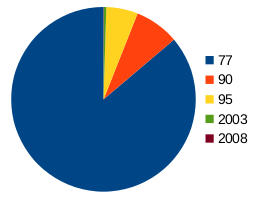
\includegraphics[width=0.4\textwidth]{images/cp2k-fortran-versions.png}
\end{center}
\caption{Usage of Language Features by Version}
\label{fig:fortran-versions}
\end{figure}

%TODO: NOTES: missing id hacks, interprocedural analysis discussion, library file/module discussion, ...?
\subsection{Finding OpenMP Regions Using Key Constructs}

\begin{lstlisting}[caption=foo, label=lst:foo]
select sym.name,
       count(sym.name)
from   gcc.annotated_code as annotated
       join gcc.gfc_symbol as sym
         on sym.record_address = annotated.ns_proc_name
            and sym.build_id = annotated.build_id
where  annotated."ext.omp_clauses" is not null
       and annotated.op in ( 75, 76 )
       and sym.name in (select *
                        from   subquery)
group  by sym.name
having count(sym.name) > 1
order  by count(sym.name) desc;  
\end{lstlisting}

\begin{lstlisting}[caption=foo, label=lst:bar]
select distinct code_lines.ns_proc_name.name
from	(
		select stack_files.file,
		       stack_lines.line
		from	(
				select   files,
				         lines
				from     map.stack_line_frequency
				group by files,
				         lines limit 1) stack
		join   unnest(stack.files) with ordinality as stack_files(file, index)
		on     true
		join   unnest(stack.lines) with ordinality as stack_lines(line, index)
		on     stack_lines.index = stack_files.index
		join	(
				select distinct filename
				from            gcc.gfc_file) file
		on     file.filename = stack_files.file) freq
join	gcc.code_lines as code_lines
on	code_lines.filename = freq.file
and	code_lines.lines @> array[freq.line]
join	gcc.gfc_symbol as sym
on	sym.record_address = code_lines.ns_proc_name
and	sym.build_id = code_lines.build_id;
\end{lstlisting}

\begin{table}[htbp]
\caption{ScaLAPACK Subroutine Reference Locations}
\begin{center}
\begin{tabular}{|c|c|c|}
\hline
\textbf{Subroutine} & \textbf{Parallel Regions} \\
\hline
xc\_calc\_2nd\_deriv & 28 \\
\hline
xc\_rho\_set\_update & 15 \\
\hline
rs\_pw\_transfer\_distributed & 14 \\
\hline
pw\_axpy & 14 \\
\hline
mp2\_redistribute\_gamma & 12 \\
\hline
calculate\_dispersion\_nonloc & 11 \\
\hline
xc\_vxc\_pw\_create & 10 \\
\hline
rpa\_num\_int & 10 \\
\hline
pw\_spline3\_deriv\_g & 9 \\
\hline
pw\_spline2\_deriv\_g & 9 \\
\hline
pw\_copy & 8 \\
\hline
arnoldi & 8 \\
\hline
multiply\_3d & 7 \\
\hline
pw\_derive & 7 \\
\hline
sccs & 6 \\
\hline
\end{tabular}
\label{tab:foo}
\end{center}
\end{table}

%\subsection{Finding Unnecessary or Inefficient OpenMP Regions}

\subsection{Measuring Variable Use Within OpenMP Parallel Regions}

Figure~\ref{fig:openmp-refcount}

\begin{figure}
\begin{center}
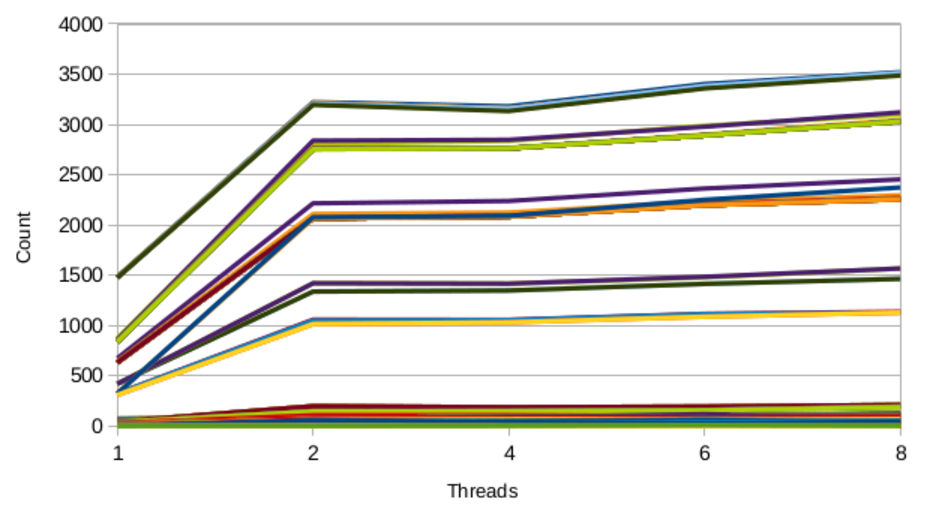
\includegraphics[width=0.4\textwidth]{images/cp2k-omp-inc-full.pdf}
\end{center}
\caption{Sampled Reference Counts to Variables Within OpenMP Parallel Regions}
\label{fig:openmp-refcount}
\end{figure}
